\chapter{Surface current on the waveguide 
walls}
In our recent discussions, we embarked on a fascinating journey through the realm of electromagnetic wave propagation within waveguiding structures. Our exploration took us through the intricacies of two distinct waveguide configurations: the parallel plane waveguide and the rectangular waveguide. Each of these waveguides unfolded its unique characteristics and posed intriguing questions that demanded answers.

Let's start by delving into our initial investigations within the parallel plane waveguide. Here, we visualized the propagation of electromagnetic waves as the continuous reflection of uniform plane waves at the boundaries of the guide. This visual approach granted us an intuitive understanding of the fields that could exist within such a structure. We realized that waves propagating along the plane exhibited a traveling wave nature, while those perpendicular to the planes resembled standing waves. In contrast, our journey within the rectangular waveguide followed a mathematical path. We sought to determine the transverse electric (TE) and transverse magnetic (TM) fields by solving the wave equation while satisfying boundary conditions. This approach was purely mathematical, devoid of the visual insights that the parallel plane waveguide had provided. Now, the crux of our exploration lies in establishing a mathematical connection between the fields we derived for the rectangular waveguide and those we visualized for the parallel plane waveguide. We must verify that the fields derived through mathematical rigor for the rectangular waveguide align with the physical understanding we gained from the parallel plane waveguide. One of the most intriguing questions we faced was \emph{whether the transverse electromagnetic\index{transverse electromagnetic mode} (TEM) mode, which transformed into the TEM mode in the parallel plane waveguide, could also exist in the rectangular waveguide}. To address this, we embarked on a thoughtful analysis.

To determine whether the TEM mode could thrive within the rectangular waveguide, we considered the nature of its electric and magnetic fields. In the TEM mode, both the electric and magnetic fields are perpendicular to the direction of propagation, confined to the cross-sectional plane as shown in Figure~\ref{fig:group4001}. However, a critical observation arises: magnetic field lines must form closed loops, and for this to occur, there must be an enclosed current.

Two possibilities emerge: either a conduction current flowing perpendicular to the transverse plane or a displacement current flowing in the same direction. Yet, within the hollow confines of the rectangular waveguide, where no conducting medium resides, the conduction current is nonexistent. Thus, the only remaining option is the displacement current. However, this would necessitate an electric field component perpendicular to the transverse plane, which contradicts the fundamental nature of the TEM mode.

The verdict is clear: the TEM mode cannot exist within the rectangular waveguide due to the absence of current support. This conclusion provides valuable insights into the limitations of waveguides with hollow structures.
\begin{figure}[h]
\centering
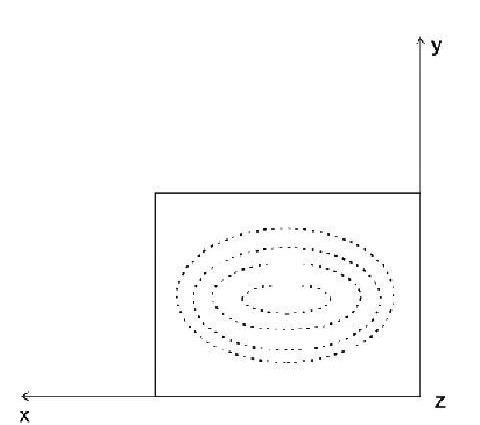
\includegraphics[width=0.6\linewidth]{\pathtoparttwo/graphics/group4001}
\caption{Field patterns of the magnetic fields on the rectangular waveguide wall in the XY plane}
\label{fig:group4001}
\end{figure}

Conversely, within the parallel plane waveguide, the TEM mode finds its sanctuary. The magnetic field lines in this infinite structure close at infinity, enclosing the conducting boundaries and supporting the required current. This makes it possible for the TEM mode to thrive in the parallel plane waveguide.

\section{Limiting Case: Parallel Plane Waveguide as Rectangular Waveguide}
Consider a rectangular waveguide where the TE$_{10}$ mode exists. In this mode, the electric field is oriented as shown in Figure~\ref{fig:page3}.Now, imagine extending one of the walls of this rectangular waveguide to infinity, effectively making `b' (the width of the guide) equal to infinity. This transformation creates a structure that resembles a parallel-plane waveguide, with two planes and wave propagation occurring in the z-direction. In this new configuration, both walls are pushed to infinity. In this context, the TE$_{10}$ mode of the rectangular waveguide becomes the TE mode in the parallel-plane waveguide by pushing one boundary to infinity.
\begin{figure}[h]
\centering
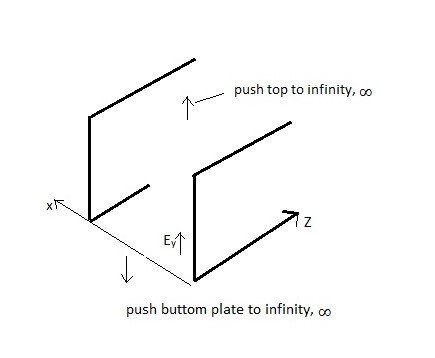
\includegraphics[width=.7\linewidth]{\pathtoparttwo/graphics/page3}
\caption{A Parallel-Plane Waveguide as the Limiting Case of a Rectangular Waveguide with $b=\infty$}
\label{fig:page3}
\end{figure}

As we extend the walls of the rectangular waveguide to infinity, we effectively metamorphose it into a parallel-plane waveguide. In this new geometry, the electric field is oriented in the y-direction, and wave propagation occurs perpendicular to the transverse plane. This mode closely resembles the TE mode. Consequently, the electric field (E) and magnetic field (H) take on the orientations described by Equations~\eqref{eqn:te10start} through~\eqref{eqn:te10end}.

\begin{align}
E_x &= E_z = H_y = 0\label{eqn:te10start}\\
E_y &= -\frac{j\omega \mu a}{\pi}C\sin(\frac{\pi x}{a})e^{-j\beta z}\\
H_x &= -\frac{j\beta a}{\pi}C\sin(\frac{\pi x}{a})e^{-j\beta z}\\
H_z &= C\cos(\frac{\pi x}{a})e^{-j\beta z}\label{eqn:te10end}
\end{align}

Notably, in this case, both magnetic field components, $H_x$ and $H_z$, coexist, and all these fields remain constant with respect to the y-coordinate.

With $b=\infty$, we encounter an intriguing scenario: there are no boundary conditions to impose in the y-direction. Consequently, the electric field $E_y$ remains constant along the y-direction. Remarkably, this aligns precisely with the electric field observed in a parallel-plane waveguide. Therefore, for a rectangular waveguide operating in the TE$_{10}$ mode with $b=\infty$, the fields essentially mirror those of a parallel-plane waveguide operating in the TE$_1$ mode. This equivalency implies that the TE$_1$ mode of a parallel-plane waveguide shares identical field characteristics with the TE$_{10}$ mode of a rectangular waveguide, both featuring a magnetic field in the z-direction.

This transition allows us to obtain the transverse electric mode, specifically the lowest-order transverse electric mode for the rectangular waveguide, which aligns perfectly with the lowest-order transverse electric mode for the parallel-plane waveguide—the TE$_1$ mode.

Now, let's shift our focus to the Transverse Electromagnetic Mode. In TEM mode within the parallel-plane waveguide, the electric and magnetic field patterns are illustrated in Figure~\ref{fig:page4}.

\begin{figure}[h]
\centering
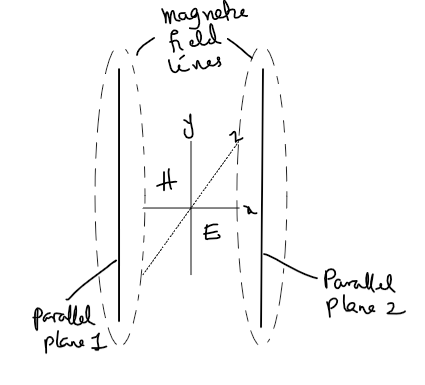
\includegraphics[width=.7\linewidth]{\pathtoparttwo/graphics/surface_current_parallel_plane_wg_temp}
\caption{Field Patterns and Surface Currents for the Electric and Magnetic Fields in a Parallel-Plane Waveguide Operating in TEM Mode}
\label{fig:page4}
\end{figure}

Notably, in TEM mode, the wave travels without any variation in the electric and magnetic fields. This occurs because neither the tangential components of the magnetic field require boundary conditions to be satisfied (which permits surface currents), nor do the normal components of the electric field require specific boundary conditions. In the latter case, surface charges can be induced to compensate for any discrepancies. Consequently, TEM mode thrives within the parallel-plane waveguide.

At this juncture, a pertinent question arises: \emph{if Figure~\ref{fig:page4} represents the limiting case of the rectangular waveguide, why does TEM mode flourish within parallel-plane waveguides but remain absent in rectangular waveguides?} The answer lies in the orientation of the magnetic field. In parallel-plane waveguides, where the magnetic field aligns with the y-direction and the planes extend infinitely along this axis, the magnetic field lines effectively close at infinity, enclosing the conducting walls, as depicted by the dotted lines. Consequently, surface currents flow along these conducting planes. In contrast, within the finite boundaries of a rectangular waveguide, the magnetic field lines close upon themselves, resulting in no enclosed current. This fundamental distinction explains why TEM mode cannot thrive within rectangular waveguides but can flourish in the presence of a parallel-plane structure. The magnetic field lines extend to infinity, thereby enclosing the plane conductors, as illustrated in Figure~\ref{fig:page4}. This unique feature allows TEM mode to thrive within parallel-plane waveguides, making it the ideal choice for certain applications, such as in the case of two-conductor systems like coaxial cables.

In summary, the propagation of TEM mode, characterized by its non-dispersive behavior, represents a defining feature of parallel-plane waveguides. However, it is essential to acknowledge that parallel-plane waveguides are not practical for real-world applications due to their infinite extent. In practical scenarios, rectangular waveguides are the go-to choice, but they introduce constraints and challenges, including dispersion and cutoff frequencies. These limitations need to be carefully considered when designing waveguide systems.


\section{Currents and Fields in Waveguides}
In the study of waveguides and electromagnetic fields, it is crucial to comprehend the complex relationship between currents and charges, as they are the fundamental elements that support the propagation of electromagnetic waves. In this exploration, we will delve into the currents excited on the walls of a waveguide and their role in maintaining the electromagnetic fields within. These fields are responsible for carrying power through the waveguide, making them fundamental to waveguide theory.

Whether we are dealing with a parallel-plane waveguide or a rectangular waveguide, the mechanism that sustains electromagnetic fields within these structures relies on the presence of sources. These sources, in this context, are surface charges and surface currents residing on the inner surface of the waveguide.

As electromagnetic waves travel through the waveguide, these surface charges and currents continuously move and redistribute themselves along the inner walls. Their presence and dynamics are essential in supporting the electric and magnetic fields that form the foundation of waveguide-based communication and transmission systems.

To comprehend this intricate interplay between currents and fields, let's begin by visualizing the fields within a waveguide, focusing on the simplest case: the Transverse Electromagnetic (TEM) mode in a parallel-plane waveguide.

\subsection{TEM mode}
In the TEM mode, the electric field and magnetic field vary harmonically with time. Considering the parallel-plane waveguide in Figure~\ref{fig:page6}, we can express these fields as
\begin{align*}
E_y = Ce^{-j\beta z}e^{j\omega t}\\
H_x = {\frac{C}{\eta}}e^{-j\beta z} e^{j\omega t}
\end{align*}
\begin{figure}[h]
\centering
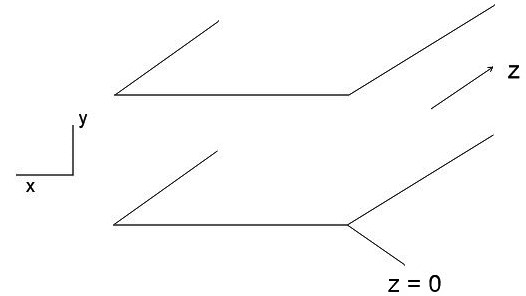
\includegraphics[width=.7\linewidth]{\pathtoparttwo/graphics/page6}
\caption{Parallel Plane waveguide}
\label{fig:page6}
\end{figure}

However, to understand their spatial distribution, we freeze time, effectively removing the time-dependent harmonic component (\(e^{j\omega t}\)). This allows us to concentrate on the spatial characteristics of these fields.

At this moment in time, then the field visualzation for \(E_y\) becomes \({\mathfrak{Re}\left\{Ce^{-j\beta z}\right\}}= C \cos(\beta z)\), and \(H_x\) takes the form \({\mathfrak{Re}\left\{C/\eta e^{-j\beta z}\right\}} = C/\eta \cos(\beta z)\). Here, \(C\) represents the amplitude of these fields, \(\beta\) is the phase constant, and \(\eta\) is the intrinsic impedance of the medium.

Imagine standing within the waveguide and observing the field distribution. At \(z = 0\), both the electric and magnetic fields reach their maximum amplitudes, and they remain constant in the \(x\) and \(y\) directions. As you move along the \(z\)-direction, these fields exhibit a cosine-like variation, with maxima occurring at multiples of the guide wavelength, \(\lambda_g/4\) (see Figure~\ref{fig:group4002}).

The electric field alternates between positive and negative maxima (see Figure~\ref{fig:page702}), while the magnetic field maintains its horizontal orientation with consistent amplitude throughout (see Figure~\ref{fig:page703}). This alternating pattern continues as you progress along the \(z\)-axis: maximum, zero, reversal of direction, maximum, and so on.

\begin{figure}[h]
\centering
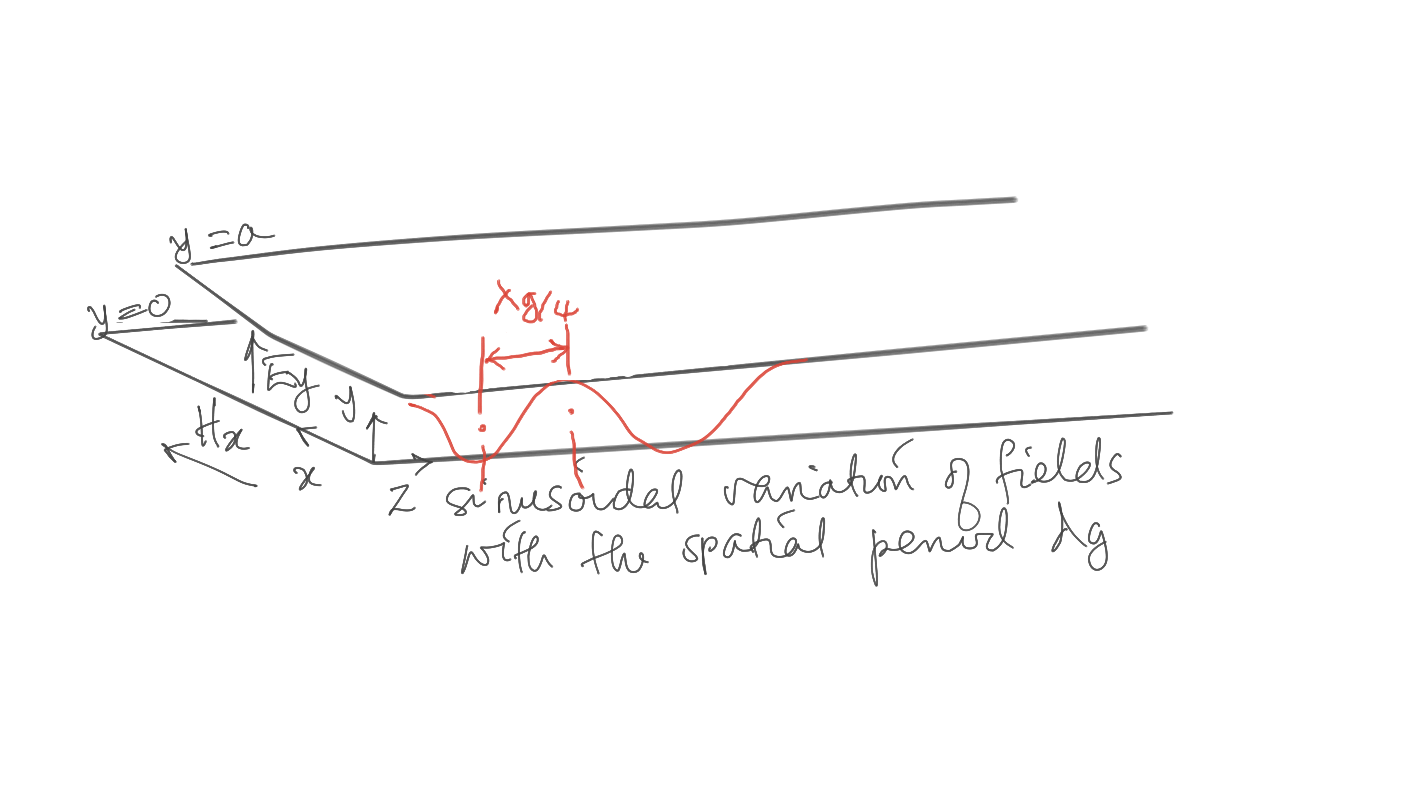
\includegraphics[width=.7\linewidth]{\pathtoparttwo/graphics/sinusoidal_variations_electric_and_magnetic_fields_temp}
\caption{Variation of the electric and magnetic field along the direction of wave propagation in TEM mode}
\label{fig:group4002}
\end{figure}
\begin{figure}[h]
\centering
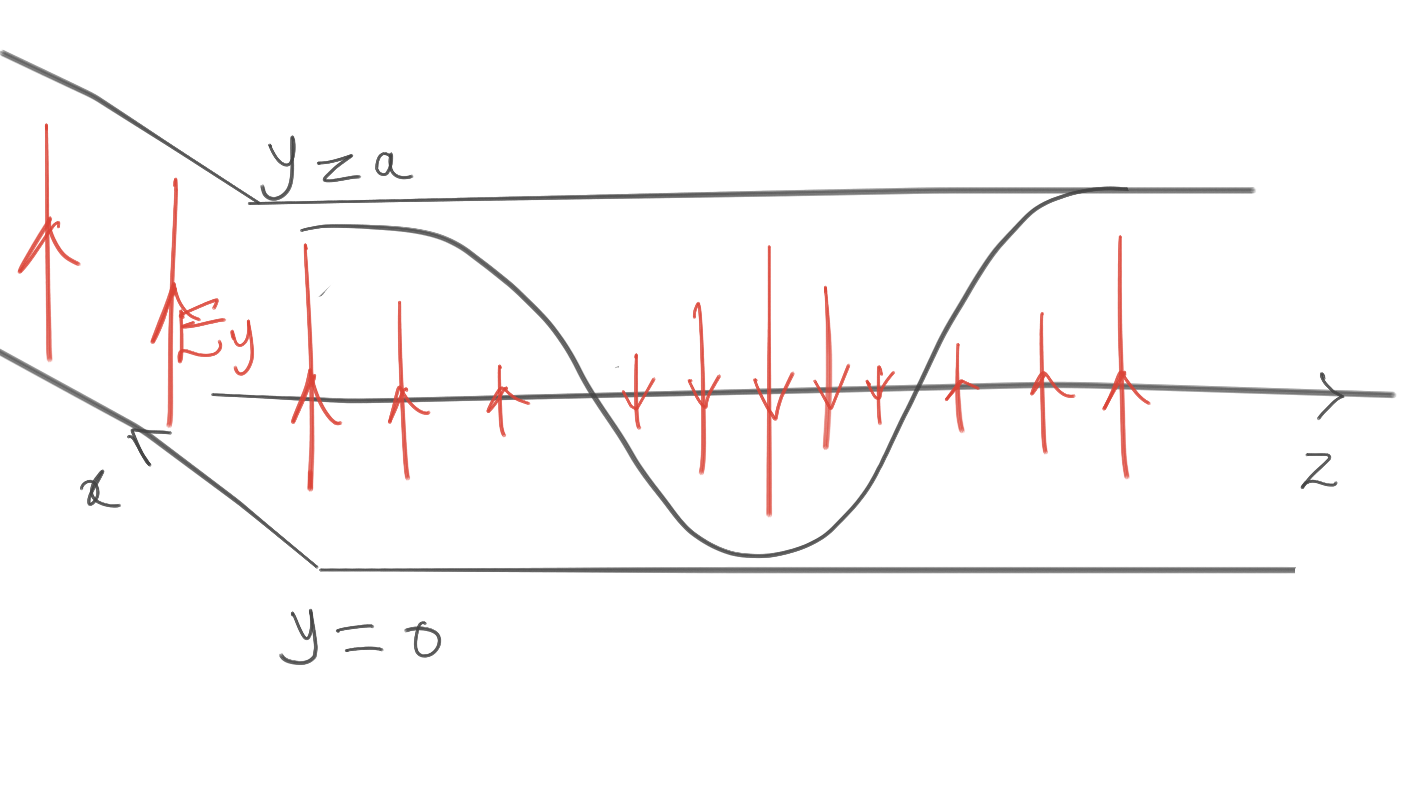
\includegraphics[width=.7\linewidth]{\pathtoparttwo/graphics/electric_field_variations_temp}
\caption{Electric field variation in a parallel plane waveguide in the TEM mode}
\label{fig:page702}
\end{figure}
\begin{figure}[h]
\centering
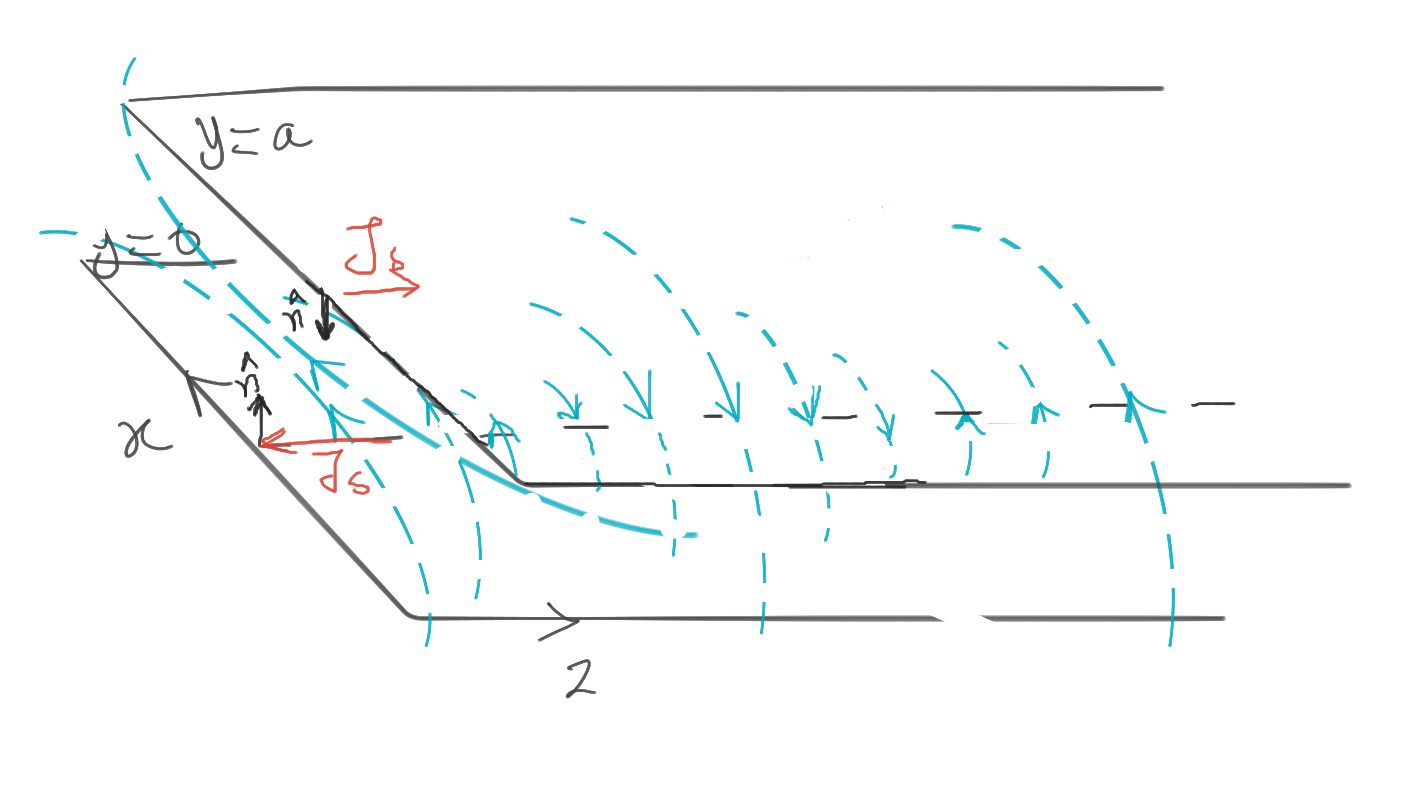
\includegraphics[width=.7\linewidth]{\pathtoparttwo/graphics/magnetic_field_variations_temp}
\caption{Magnetic field variation showing normal to parallel plane waveguide surface and surface currents in TEM mode}
\label{fig:page703}
\end{figure}

Now, let's establish a connection between the magnetic field's direction and the surface currents on the waveguide's walls. The tangential component of the magnetic field (\(H\)) is responsible for inducing surface currents on the conducting walls.

On the upper plane of the waveguide, the normal unit vector (\(\hat{n}\)) points in the \(+y\) direction. When we calculate \(\hat{n} \times \boldsymbol{H}\), we find that the surface current, \(\boldsymbol{J_s}\), flows in the direction of wave propagation (\(z\)-direction). Conversely, on the lower plane, where \(\hat{n}\) points in the \(-y\) direction, the surface current flows in the opposite direction, \(-z\). These depictions are shown in Figure~\ref{fig:page703}.

These surface currents exhibit the same spatial variation as the magnetic field, with maxima at multiples of \(\lambda_g/4\). In a two-conductor system like a coaxial cable, we observe that the current flows in the direction of wave propagation. This alignment between current flow and wave propagation direction is a characteristic of the TEM mode.

However, it's crucial to note that this alignment between current direction and wave propagation is not a universal rule. It's a characteristic of the TEM mode, which we often encounter in low-frequency circuits. In other scenarios, such as when dealing with more complex electromagnetic modes, this alignment may not hold true.

\subsection{TE mode}\index{transverse electric mode}
Let's begin by considering the TE$_1$ mode in a parallel-plane waveguide. The structure in question is depicted Figure~\ref{fig:watson4}, where we have the magnetic_field_variation mode within the parallel-plane waveguide.
\begin{figure}[h]
\centering
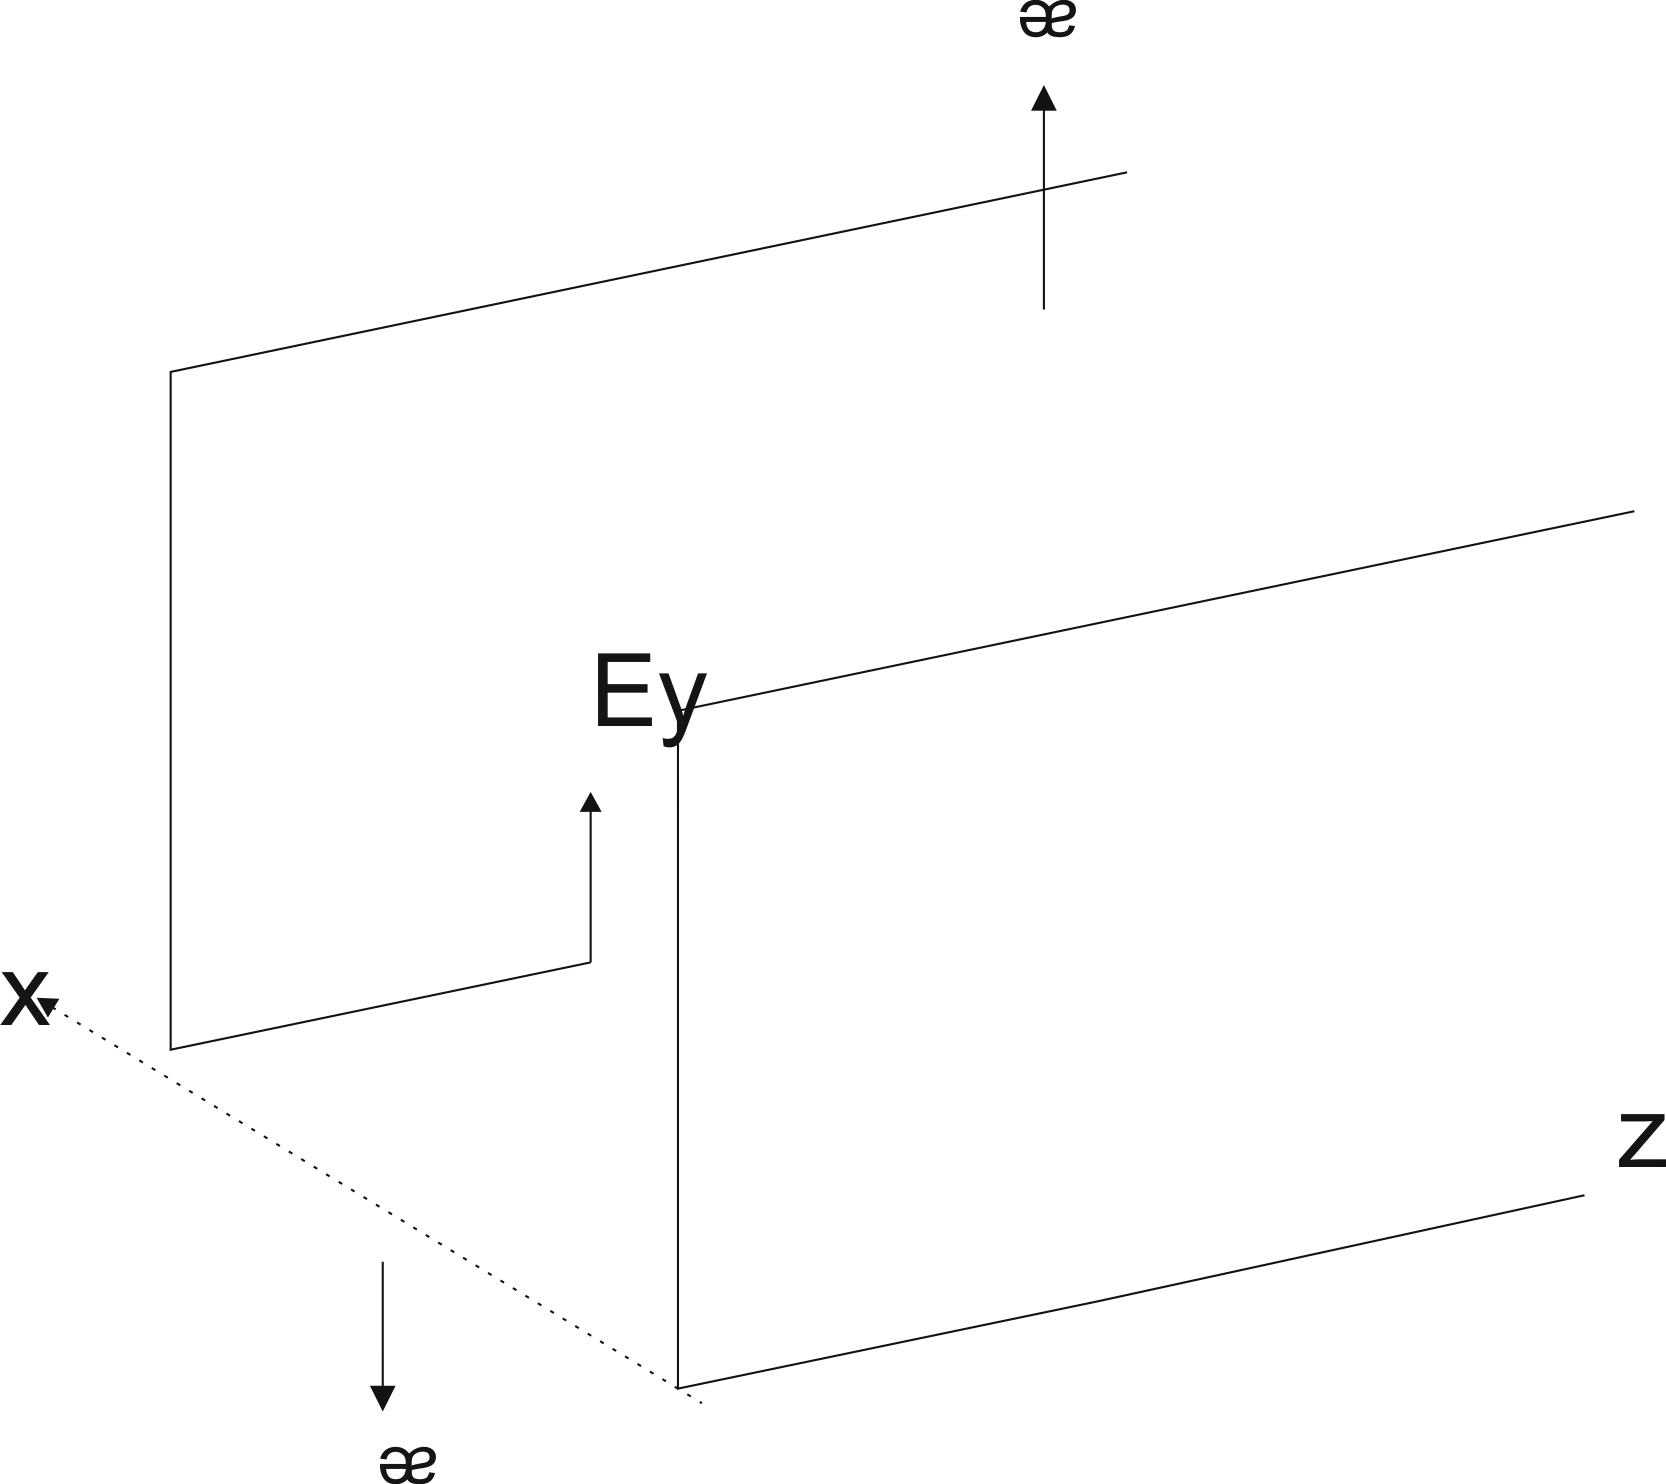
\includegraphics[width=.7\linewidth]{\pathtoparttwo/graphics/WATSON4}
\caption{Analysis of parallel plane waveguide propagating wave in the TE$_1$ mode}
\label{fig:watson4}
\end{figure}

As we've seen before, the field distribution in a parallel-plane waveguide is identical to that of the TE$_{10}$ mode in a rectangular waveguide given in Equations~\eqref{eqn:te10start}\textemdash~\eqref{eqn:te10end}

First and foremost, the electric field will be oriented in the y-direction, and it will exhibit variations in both the x and z directions, characterized by the phase constant \(\beta\). To visualize these fields effectively, we will consider their amplitudes, specifically the real parts, and plot them as functions of x, y, and z. This will allow us to create a three-dimensional representation of these fields.

Before proceeding further, we will simplify the expression for the electric field by handling the complex component represented by `-j' We know that `-j' can be expressed as $e^{-j\pi/2}$. Thus, the electric field expression can be rewritten as:
\begin{dmath*}
E_y = \dfrac{-j\omega\mu a}{\pi}C\sin(\dfrac{\pi x}{a})e^{
-j\beta z}
=e^{-j\dfrac{\pi}{2}}\times\dfrac{\omega \mu a}{\pi}C\sin(\dfrac{\pi x}{a})e^{-j\beta z}
= \dfrac{\omega \mu a}{\pi}C\sin(\dfrac{\pi x}{a})e^{-j\left(\beta z + \dfrac{\pi}{2}\right)
}
\end{dmath*}
\begin{dmath*}
\mathfrak{Re}\left\{E_y\right\} = \dfrac{\omega \mu a}{a}C\sin(\dfrac{\pi x}{a})\cos(\beta z + \dfrac{\pi}{2})
\end{dmath*}
Recall, $\cos(-\left(\beta z + \dfrac{\pi}{2}\right))=\cos(\beta z + \frac{\pi}{2})$, i.e. cosine is an even function and let ${\dfrac{\omega \mu aC}{\pi}\equiv A}$, thus we have 
\begin{dmath*}
\mathfrak{Re}\left\{E_y\right\} = A\sin(\dfrac{\pi x}{a})\cos(\beta z +\dfrac{\pi}{2}) = A\sin(\dfrac{\pi x}{a})\sin(\beta z) = A\sin(\dfrac{\pi x}{a})\sin(\dfrac{2\pi z}{\lambda_g})
\end{dmath*}
We apply a similar process to the magnetic field (H) expression, resulting in:
\begin{align*}
\mathfrak{Re}\{H_x\} = B\sin(\frac{\pi x}{a})\sin(\frac{2\pi z}{\lambda_g})\\
\mathfrak{Re}\{H_z\}= C\cos(\frac{\pi x}{a})\cos(\frac{2\pi z}{\lambda_g})
\end{align*}
These expressions represent the field distributions at a specific instant (t = 0) along the waveguide.

In the z-direction, both the electric and magnetic fields exhibit sinusoidal variations with a spatial period of $\lambda_g$. However, they are out of phase with each other. Where $H_x$ is at its maximum, $H_z$ is zero, and vice versa. This results in a two-component field system, $H_x$ and $H_z$. Let's examine their spatial behaviour:

The $H_x$ component follows a sine variation in the z-direction, with maximum amplitude at $z = \frac{\lambda_g}{4}$. As we move a distance of $\frac{\lambda_g}{2}$ along the z-axis, $H_x$ becomes maximum again. 
% add figure showing the spatial variation of Hz along the z-axis
\begin{figure}[h]
\centering
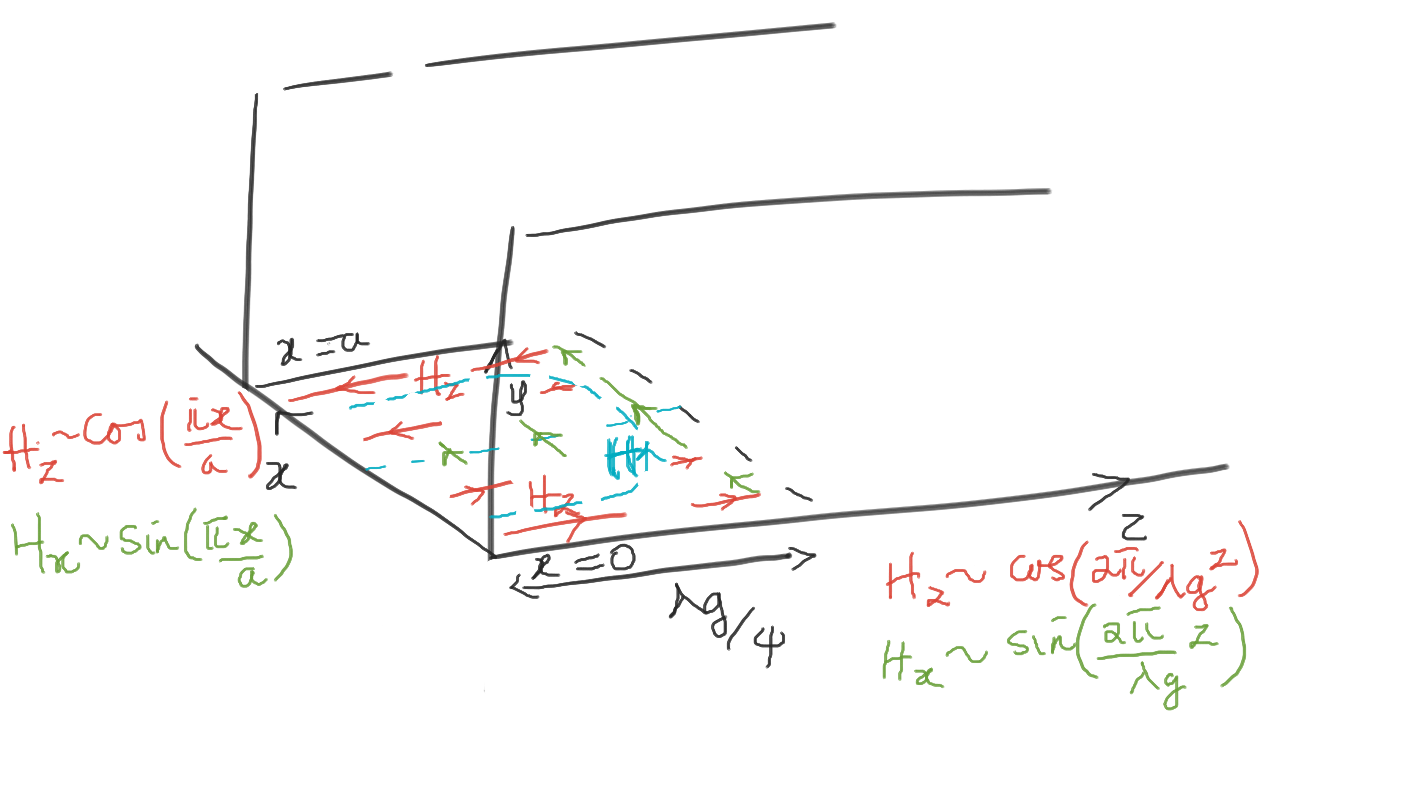
\includegraphics[width=1\linewidth]{\pathtoparttwo/graphics/magnetic_field_variations_te1_1_temp}
\caption{Magnetic field patterns showing the vector field for the components in one half cycle of the sinusoidal variations in the parallel plane waveguide operating in the TE mode}
\label{fig:watson}
\end{figure}

A view from the top of this parallel plane waveguide, shows that the magnetic field lines take the form of stacked, rolled carpets perpendicular to the plane of the paper, extending infinitely in length as shown in Figure~\ref{fig:magnetic_field_variation}.
% add figure depicting the magnetic field lines in the parallel plane waveguide
\begin{figure}[h]
\centering
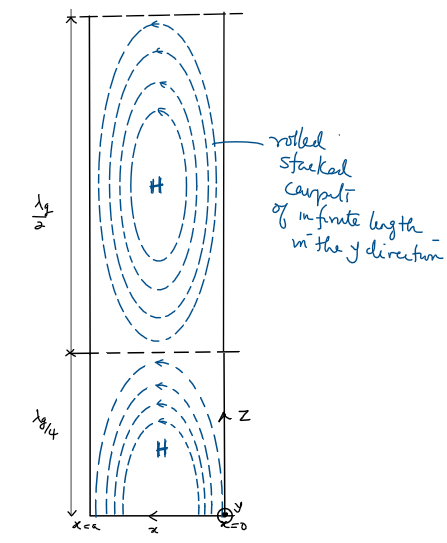
\includegraphics[width=1\linewidth]{\pathtoparttwo/graphics/magnetic_field_variations_te1_2_temp}
\caption{Resulting Magnetic field patterns in the parallel plane waveguide operating in the TE mode}
\label{fig:magnetic_field_variation}
\end{figure}

Now, let's shift our attention to the electric field ($E_y$). It possesses a sinusoidal variation along the z-direction, similar to $H_x$, but is oriented in the y-direction.
\begin{align*}
E_y= A\sin(\dfrac{\pi x}{a})\sin(\dfrac{2\pi z}{\lambda_g})
\end{align*}
Consequently, the electric field lines are perpendicular to the plane of the paper, with their amplitudes varying as the distance from the center increases.
% add figure depictin the electric field lines in the parallel plane waveguide
\begin{figure}[h]
\centering
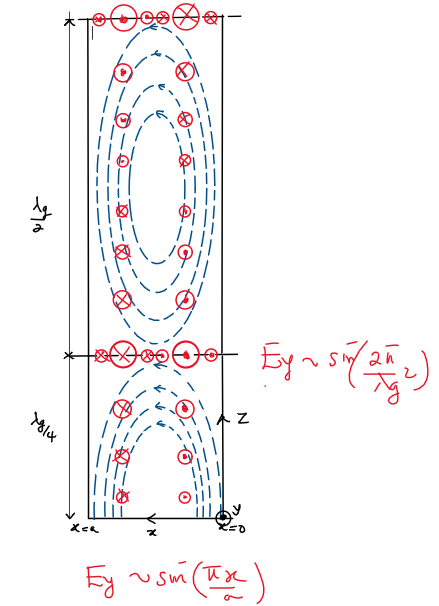
\includegraphics[width=1\linewidth]{\pathtoparttwo/graphics/electric_field_variations_te1_temp}
\caption{Electric field variation in the parallel plane waveguide operating in the TE$_1$ mode}
\label{fig:electric_field_variation}
\end{figure}

With a clear picture of the field distributions, let's explore the currents generated on the waveguide's surface. These currents are determined by the tangential component of the magnetic field on the walls.

For the leftside wall, where the magnetic field has only a z-component, the normal unit vector $\hat{n}$ points inward along the +x direction. Therefore, when calculating $\hat{n} \times \boldsymbol{H}$, the resulting current flows in the y-direction. Conversely, on the rightside wall, where the magnetic field has no x-component, the normal unit vector $\hat{n}$ points inward along the -x direction. Consequently, the surface current flows in the opposite y-direction (see Figure~\ref{fig:surface_current_variation}).
% add figure depicting the direction of surface current (Js) on the walls of the parallel plane waveguide
\begin{figure}[h]
\centering
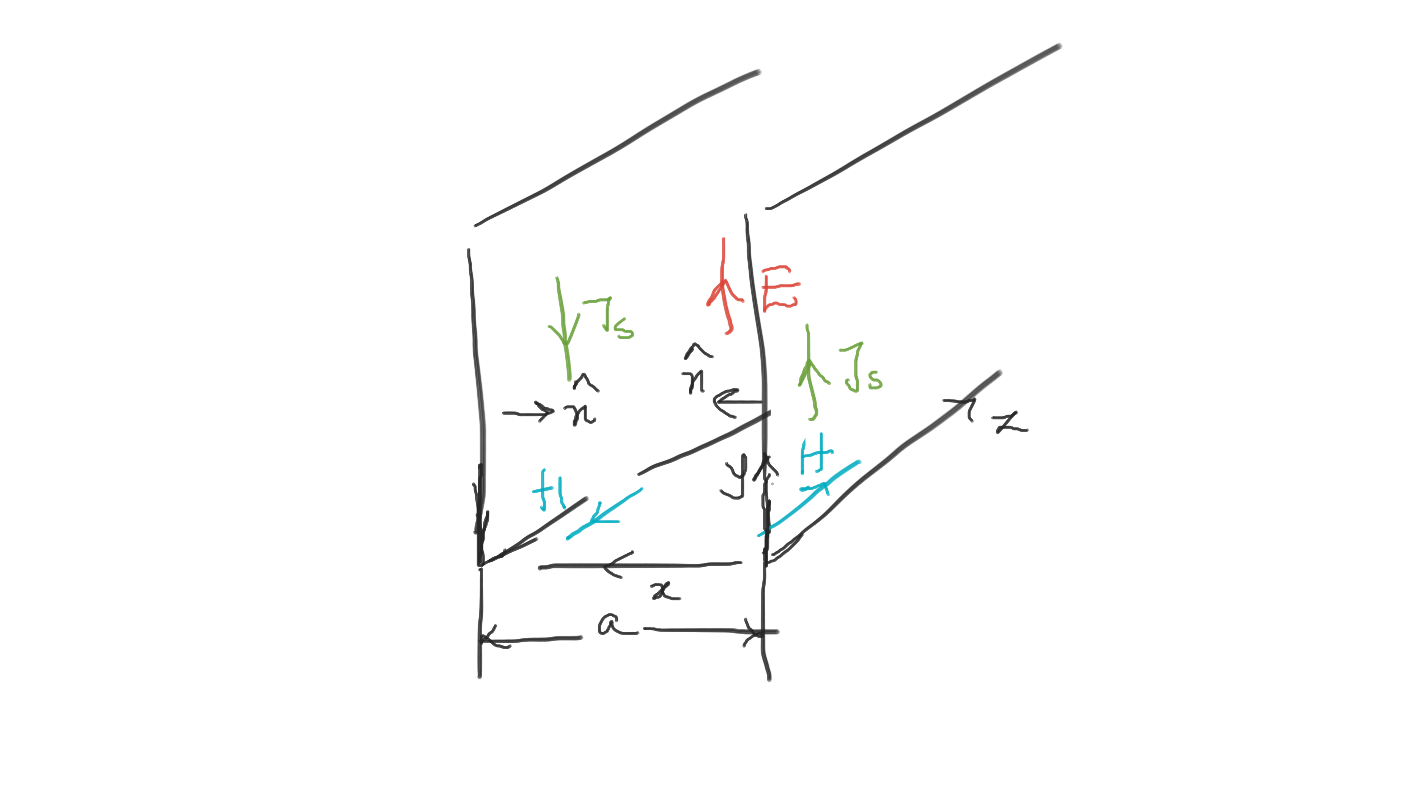
\includegraphics[width=1\linewidth]{\pathtoparttwo/graphics/surface_current_variations_te1_temp}
\caption{Surface current variations in the parallel plane waveguide operating in the TE$_1$ mode}
\label{fig:surface_current_variation}
\end{figure}

Notably, in contrast to the TEM mode, where the current and power flow coincide, in this scenario, the surface current flows perpendicular to the direction of power flow. While the current flows in the y-direction, the power flows in the z-direction. This highlights an essential distinction: the direction of current and power flow can be independent of each other.

In summary, our exploration has shed light on the intricate interplay of fields and currents within a parallel-plane waveguide, specifically in the TE1 mode. We've uncovered the unique spatial patterns of electric and magnetic fields and how they relate to surface currents. Additionally, we've challenged the conventional notion that current and power flow must align, emphasizing that they can have distinct directions.

This understanding serves as a foundational concept in the realm of electromagnetic wave propagation and waveguide theory, enriching our comprehension of complex electromagnetic phenomena. It also highlights the importance of considering different modes and configurations in the study of electromagnetic fields.

Next, we will delve into the field distribution and current flow within a rectangular waveguide, a practical structure commonly used in waveguide applications. We will also explore advanced topics, such as calculating losses in waveguides.

\section*{Exercises}
\begin{ExerciseList}
\Exercise[label={ex401}]
Can the Transverse Electromagnetic (TEM) mode exist within a rectangular waveguide, and if not, what are the underlying reasons for its absence?
\Exercise[label={ex402}]
Describe the field patterns and current distributions in the Transverse Electromagnetic (TEM) mode within a parallel-plane waveguide, and explain why this mode is supported in such a structure.
\Exercise[label={ex403}]
In the context of parallel-plane waveguides and rectangular waveguides, why does the alignment between current direction and power flow direction differ, and what does this reveal about the interplay between fields and currents in waveguide systems?
\end{ExerciseList}
